\tikzset{
	bronche/.style={
		double distance=1cm,
		double=pink,
		thick
	}
}
	\begin{columns}[T, onlytextwidth]
		\column{0.4\textwidth}
		\begin{block}{Débit laminailre}
	\begin{tikzpicture}[
			every pin/.style={
				font=\scriptsize
			},
			]
		\draw [
			bronche,
		]
		(.5,0) -- (.5, -3.35) node [midway, minimum width=1.1cm,
		pin=0:{(Ceci est une bronche !)}] {};
		%\draw (0,0) -- (0,-3.25);
		%\draw (1,0) -- (1,-3.25);
		\shade[
			left color   = bleuclairchum,
			right color  = bleuclairchum,
			middle color = marinechum,
			rounded corners
		]
		(0,0) -- (0.5,-3) --  (1,0);
		\node [white] at(0.5, -1) {$\downarrow$};
		\node [white] at(0.25, -.5) {$\downarrow$};
		\node [white] at(0.75, -.5) {$\downarrow$};
		\node [white] at(0.5, -2) {$\downarrow$};
	\end{tikzpicture}
	\end{block}

		\column{0.4\textwidth}
		\begin{block}{Débit turbulent}
	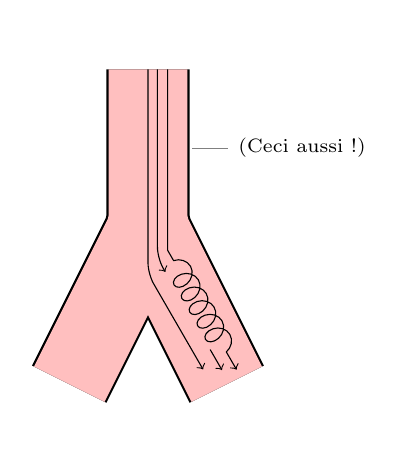
\begin{tikzpicture}[
			every pin/.style={
				font=\scriptsize
			},
			]
			\draw [
				bronche,
				rounded corners,
			] (0,0) -- (0,-2) node [midway, minimum width=1.1cm, pin=0:{(Ceci
			aussi !)}] {}--
			++(1, -2) (0,0) -- (0,-2) -- ++(-1,-2);
			\draw [->, rounded corners] (0,0) -- ++(-90:2.6) -- ++(-60:1.4) ;
			\draw [->, rounded corners] (.12,0) -- ++(-90:2.4) -- ++(-60:.2) ;
			\draw [
				->,
				decoration={
					coil,
					amplitude=1.5mm,
					aspect=.8,
					segment length=2mm,
					pre length=1.5mm,
					post length=1.5mm,
				}
			]  
			(.25,0) -- ++(-90:2.3) decorate {-- ++(-60:1.75)} ;
			\draw [->, rounded corners] (.12,0) ++(-90:2.4) ++(-60:1.34) --
			++(-60:.3);
	\end{tikzpicture}
		\end{block}
	\end{columns}
